\section{The Standard Model} \label{sec:theory:standardmodel}

At the turn of the 20th century our understaning of the constituent matter of
the universe was limited to what we could see with microscopes and imply from
the observations of light and elctricity, giving us evidence for both the photon
and the electron.  In the first half of the century we discovered the field of
subatomic physics with Rutherfords 1911 gold foil scattering experiment, and
Dirac successfully demonstrated the quantization of the electromagnetic field,
the first step towards a fully Gauge Invariant Quantum Field Theory.
In the second half we literally delved deeper, discovering that the nucleus
contained structure and extended our theories to include the the complex
mechanics of quarks and gluons.  With the discovery of the Higgs in 2013 the
Standard Model has become an irrefutable framework as can be seen in the high
level of agreement betwee theory experiment in figure \ref{fig:comparison}.

\begin{figure}[!htbp]
  \begin{center}
    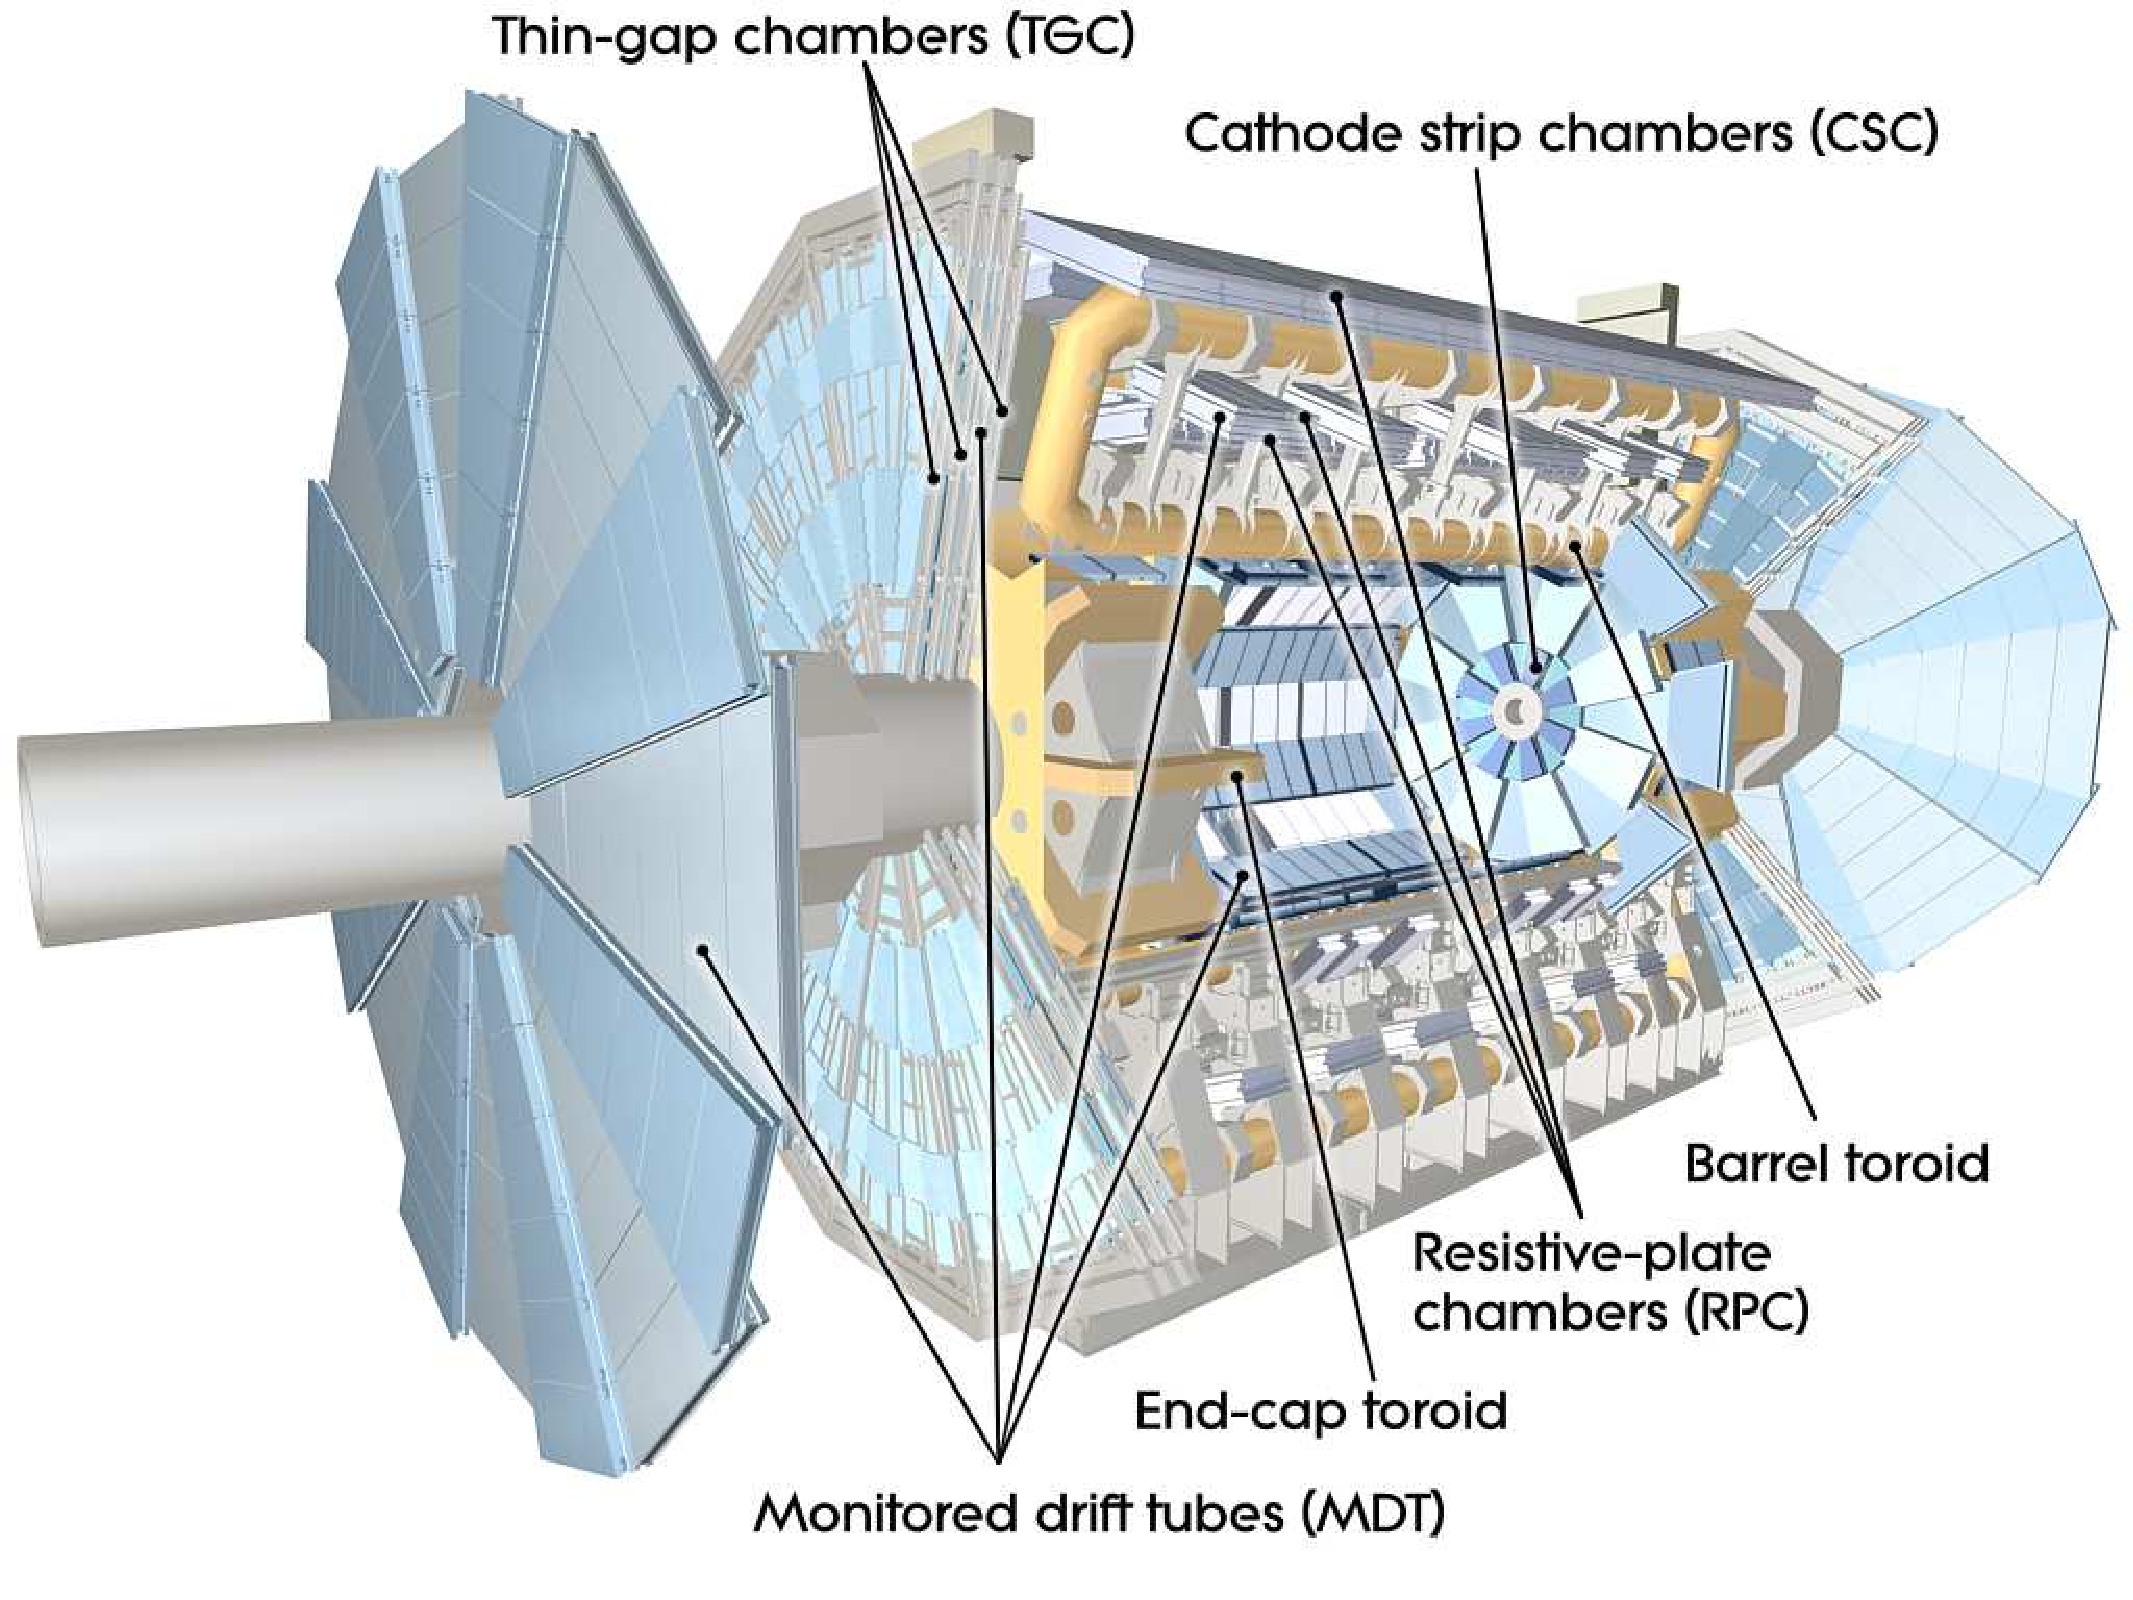
\includegraphics[width=0.8\linewidth]{figures/atlas/muon_system}
    \caption{ \cite{PERF-2007-01} A cut-away diagram of the ATLAS muon system
and its many sub-detectors.}
    \label{fig:muon_system}
  \end{center}
\end{figure}

The QCD and QED theories predict two classes of particles: fermions and
bosons. These particles represent the quanta of the quantum fields of the
Standard Model and and the mediators of the fundamental forces of Nature.

